\documentclass[11pt,letterpaper]{article}
\usepackage[margin=0.65in,footskip=0.28in]{geometry}
\usepackage[T1]{fontenc}
\usepackage[table]{xcolor}
\usepackage{helvet,microtype,array,tabularx,enumitem,fancyhdr,tikz}
\usepackage{hyperref}
\usetikzlibrary{arrows.meta}
\renewcommand{\familydefault}{\sfdefault}
\definecolor{ink}{HTML}{222222}
\definecolor{linkblue}{HTML}{245B87}
\definecolor{grid}{HTML}{D9D9D9}
\definecolor{head}{HTML}{30343A}
\definecolor{stripe}{HTML}{F3F4F5}
\hypersetup{colorlinks=true,urlcolor=linkblue,linkcolor=linkblue,pdftitle={Our sound setup},pdfauthor={Howard Wang}}
\setlength{\parindent}{0pt}
\setlength{\parskip}{5pt}
\setlength{\tabcolsep}{5pt}
\renewcommand{\arraystretch}{1.15}
\setlength{\extrarowheight}{2.5pt}
\renewcommand{\tabularxcolumn}[1]{m{#1}}
\arrayrulecolor{grid}
\newcolumntype{L}{>{\raggedright\arraybackslash}X}
\newcolumntype{P}[1]{>{\raggedright\arraybackslash}m{#1}}
\newcolumntype{C}[1]{>{\centering\arraybackslash}m{#1}}
\newcommand{\sectiontitle}[1]{\par\vspace{7pt}{\large\bfseries #1}\par\vspace{2pt}}
\pagestyle{fancy}\fancyhf{}
\fancyfoot[R]{\fontsize{9}{11}\selectfont M50 sound setup\enspace |\enspace\thepage}
\renewcommand{\headrulewidth}{0pt}
\begin{document}
\raggedright
{\fontsize{24}{28}\selectfont Our sound setup}\par
{\itshape Parts and setup\enspace |\enspace 16 October 2026}\par
\textbf{Goal:} play and measure approximately 1.4--32 kHz tones, changing every 10 ms. Check the sound setup on the mouse rig first, then recalibrate for sheep.
\sectiontitle{What to get}
{\rowcolors{2}{white}{stripe}
\begin{tabularx}{\linewidth}{|P{1.94in}|L|C{0.25in}|C{0.81in}|}\hline
\rowcolor{head}\color{white}\textbf{Part and buying link} & \color{white}\textbf{Other options and why this fits} & \color{white}\textbf{Qty} & \color{white}\textbf{Cost}\\\hline
\href{https://www.bhphotovideo.com/c/product/359562-REG/Earthworks_M50_M50_Measurment_Microphone.html}{Earthworks M50} & UMIK-2 factory calibration stops at 20 kHz; M30 G2 calibration at 32 kHz is unconfirmed. M50 offers a 50 kHz range and individual calibration with our Mac interface. & 1 & \$1,299.00 \\\hline
\href{https://www.bhphotovideo.com/c/product/1641632-REG/audient_id14_mkii_2_channel_usb2_interface_and.html}{Audient iD14 MKII} & iD4 can do the basic sound checkout, but has one full-band mic/line input. iD14 gives two for recording the mic and electrical timing reference together. & 1 & \$349.00 \\\hline
\href{https://us.edifier.com/products/mr3}{Edifier MR3 powered pair} & Original MR4 stops at 20 kHz. MR5 (\$349.99) also specifies 40 kHz. MR3 saves \$200 and covers our target on paper; 10 ms acoustic tests are still required. & 1 & \$149.99 \\\hline
\href{https://www.globaltestsupply.com/product/reed-r8090-sound-level-calibrator}{REED R8090} & Extech 407766 (\$519 listed) also provides a 1 kHz level check. R8090 costs less; both state +/-0.5 dB at 94 dB. R8090-NIST adds a certificate at extra cost. & 1 & \$219.00 \\\hline
\href{https://www.sweetwater.com/store/detail/HMIC010--hosa-hmic-010-pro-microphone-cable-rean-xlr3f-to-xlr3m-10-ft}{Hosa HMIC-010 XLR 10 ft} & Connects M50 to the interface. & 1 & \$17.99 \\\hline
\href{https://www.sweetwater.com/store/detail/HSS005--hosa-hss-005-pro-balanced-interconnect-rean-1-4-in-trs-to-same-5-foot}{Hosa HSS-005 TRS 5 ft} & One cable to the speaker; one for the electrical reference. & 2 & \$29.90 \\\hline
\href{https://www.sweetwater.com/store/detail/RIMICTPFBM--rok-it-tripod-microphone-stand-with-fixed-boom}{Gator RI-MICTP-FBM boom mic stand} & Holds the microphone at the ear position. & 1 & \$34.99 \\\hline
\end{tabularx}}
\sectiontitle{SONIC paper experiment}
Two awake, alert sheep heard tones while a 421-channel Connexus implant recorded auditory cortex. A decoder predicted the tone frequency.\par
\textbf{Benchmark stimuli:} 10 ms sine pips (100/s), zero starting phase, 2 ms ramps at both ends, and no silence between pips. Neural features used 5 ms bins.\par
\textbf{Frequencies:} Sheep C used 37 frequencies over about 1.4--32 kHz in 1/8-octave steps. Sheep E used 2, 4, 6, 8, 9, 10.5, 17, 18.2, 19.5, 20.9, 22.4, 24, 25.8 and 27 kHz.\par
\textbf{Blocks:} Uniformly random frequencies, balanced within each block. 8,000--15,000 pips per block; at least 12 blocks per session; 1 s silence between blocks.\par
\textbf{Playback:} Precomputed waveform at 192 kHz: NI USB-6361 \(\rightarrow\) TDT SA1 amplifier \(\rightarrow\) MF1 speaker; about 80 dB SPL at the sheep's ears.\par
{\fontsize{9}{11}\selectfont \href{https://doi.org/10.1101/2025.09.30.679683}{SONIC v1} --- pp. 7, 11 (\S 6.1--6.3), 13 (\S 6.6). Exact 37-frequency array and ramp shape are not listed.\par}
\newpage
{\Large\bfseries Put it together}\par
\vspace{8pt}
\begin{center}
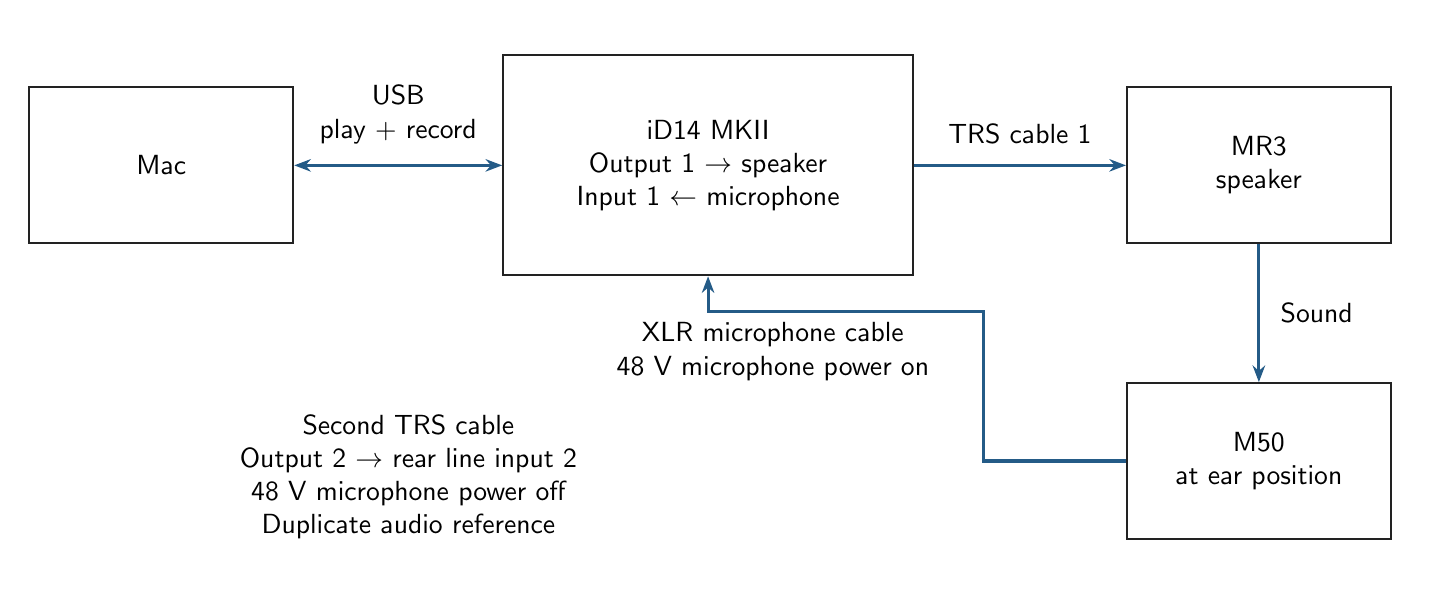
\begin{tikzpicture}[x=0.405in,y=0.405in,font=\normalsize,
 box/.style={draw=ink,line width=0.65pt,align=center,minimum width=1.32in,minimum height=0.78in},
 flow/.style={draw=linkblue,line width=1.1pt,-{Stealth[length=6pt]}}]
\path[use as bounding box] (0,0) rectangle (17,6.6);
\node[box] (mac) at (1.65,4.9) {Mac};
\node[box,minimum width=2.05in,minimum height=1.1in] (interface) at (8.4,4.9) {iD14 MKII\\Output 1 $\rightarrow$ speaker\\Input 1 $\leftarrow$ microphone};
\node[box] (speaker) at (15.2,4.9) {MR3\\speaker};
\node[box] (mic) at (15.2,1.25) {M50\\at ear position};
\draw[flow,{Stealth[length=6pt]}-{Stealth[length=6pt]}] (mac.east) -- node[above,align=center,yshift=4pt] {USB\\play + record} (interface.west);
\draw[flow] (interface.east) -- node[above,yshift=4pt] {TRS cable 1} (speaker.west);
\draw[flow] (speaker.south) -- node[right,xshift=4pt] {Sound} (mic.north);
\draw[flow] (mic.west) -- (11.8,1.25) -- (11.8,3.1) -- (8.4,3.1) -- (interface.south);
\node[align=center] at (9.2,2.6) {XLR microphone cable\\48 V microphone power on};
\node[align=center] at (4.7,1.05) {Second TRS cable\\Output 2 $\rightarrow$ rear line input 2\\48 V microphone power off\\Duplicate audio reference};
\end{tikzpicture}
\end{center}
{\fontsize{9}{11}\selectfont Connections for sound playback and recording\par}
\begin{enumerate}[leftmargin=0.24in,labelsep=0.09in,itemsep=6pt,topsep=7pt]
\item \textbf{Connect and position.} Connect as shown. Turn on 48 V microphone power for input 1; keep it off for input 2. Turn input monitoring off to prevent feedback; leave the front instrument input empty. Put the M50 tip at the ear/reference position and record distance and angle.
\item \textbf{Program the sequence.} Python builds one continuous waveform at 96 kHz: 960 samples per 10 ms pip, including a 2 ms ramp at each end. Send it to output 1 and a copy to output 2. Save the tone schedule and random seed.
\item \textbf{Calibrate.} Use the calibration file for that M50, checking coverage through 32 kHz. Use the R8090 at 94 dB to set the recording scale, then keep mic gain fixed. Remove the calibrator and adjust each tone's level using recordings at the ear position.
\item \textbf{Check the actual sound.} Record the microphone and electrical reference simultaneously during the actual 10 ms sequence. Check level at every frequency, short-tone transitions, ringing and stability through a full run. Check the reference channel's relative delay too. Repeat calibration when moving to sheep.
\end{enumerate}
\textbf{Before testing:} the lab chooses distance, sound level and pass tolerances. The paper's approximately 80 dB sheep level is not automatically the mouse setting. Physical sound checks and later neural synchronization are still pending.\par
{\fontsize{9}{11}\selectfont Specifications: \href{https://earthworksaudio.com/measurement-microphones/m50/}{M50}\enspace $\cdot$\enspace \href{https://audient.com/products/audio-interfaces/id14/tech-specs/}{iD14}\enspace $\cdot$\enspace \href{https://www.edifier.com/global/p/studio-monitors/mr3}{MR3}\enspace $\cdot$\enspace \href{https://www.reedinstruments.com/pdfs/cache/www.reedinstruments.com/r8090/datasheet/r8090-datasheet.pdf}{R8090}\par Alternatives: \href{https://www.minidsp.com/images/documents/miniDSP\%20UMIK-2-User\%20Manual.pdf}{UMIK-2}\enspace $\cdot$\enspace \href{https://earthworksaudio.com/wp-content/uploads/2025/11/Earthworks_Audio_M30_G2__11042025-1.pdf}{M30 G2}\enspace $\cdot$\enspace \href{https://audient.com/products/audio-interfaces/id4/tech-specs/}{iD4}\enspace $\cdot$\enspace \href{https://www.edifier.com/global/p/studio-monitors/mr4}{original MR4}\enspace $\cdot$\enspace \href{https://us.edifier.com/products/mr5}{MR5}\enspace $\cdot$\enspace \href{https://prod.extech.com/products/407766/}{Extech 407766}\par}
\end{document}
